\section{Etude de la stabilité du véhicule porteur}

 Le véhicule porteur de l’E.P.A.S. doit être équipé de stabilisateurs. Une fois en place, les
 stabilisateurs le soulèvent, afin qu’il ne repose plus sur les roues (les roues touchent le sol mais ne
 supportent aucun poids) : le mouvement des suspensions du véhicule mettrait en danger sa stabilité.
 
 L’objet de cette partie est de déterminer la longueur de déploiement maximale que le système de
 sécurité pourra autoriser.


\begin{figure}[H]
\centering
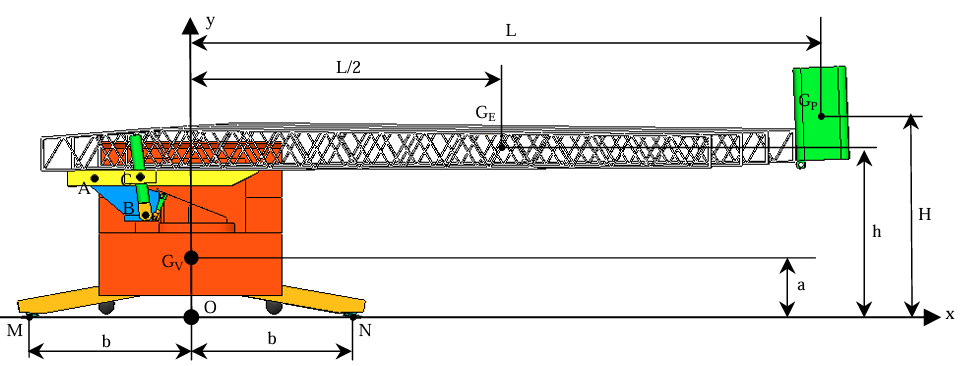
\includegraphics[width=.6\linewidth]{ccinp_psi_2007_fig_10}
\caption{\label{ccinp_psi_2007_fig_10} Stabilisateurs}
\end{figure}

 Le véhicule est dans la configuration de la figure précédente :
 \begin{itemize}
\item parc échelle horizontale;
\item stabilisateurs sortis au maximum;
\item charge maximale dans la plate-forme.
\end{itemize}


 Le problème sera traité en statique plane dans le plan $(O, x, y)$ de la figure précédente.
 
  Les efforts pris en compte sont :
  \begin{itemize}
\item les actions de pesanteur sur chaque élément.
 \end{itemize}
 
\begin{center}
\begin{tabular}{llll}
\hline
Elément & Centre d'inertie & Masse &  \\
\hline
Véhicule + charge utile & $G_V$ & $m_V$ & $\vect{OG_V}  = a\vect{y}$ \\
Parc échelle & $G_E$ & $m_E$ & $\vect{OG_E} = \dfrac{L}{2} \vect{x} + h\vect{y}$ \\
Plate forme + charge utile & $G_P$ & $m_P$ & $\vect{OG_P}=L\vect{x}+H\vect{y}$ \\
\hline
\end{tabular}
\end{center}


\begin{itemize}
\item les actions de contact de la route sur les stabilisateurs.
\end{itemize}


 Ces actions seront modélisées par des glisseurs passant l’un par $M$, tel que $\vect{OM}=-b\vect{x}$ et l’autre par $N$ tel que $\vect{ON}=b\vect{x}$.
 
 Les résultantes de ces glisseurs seront notées respectivement : $\vect{R_M} = X_M \vect{x} +  Y_M \vect{y}$ et  
 $\vect{R_N} = X_N \vect{x} +  Y_N \vect{y}$.
 


%Q23
\question{Exprimez la condition de non basculement de l’ensemble.}
 \ifprof
 \begin{corrige}
 \end{corrige}
 \else
 \fi

\question{Calculez la longueur $\indice{L}{max}$ de déploiement au-delà de laquelle il y aura basculement.}
 \ifprof
 \begin{corrige}
 \end{corrige}
 \else
 \fi
